\documentclass[12pt]{book}

\usepackage{amsfonts,amsmath,amssymb,gensymb,soul,graphicx,titlesec,tabu,longtable,array,natbib,listings,booktabs,hhline,multirow}
\usepackage[usenames,dvipsnames]{color}
\usepackage[colorlinks,linkcolor=blue,citecolor=blue,urlcolor=blue,pdftitle={Balrog},pdfauthor={Suchyta and Huff}]{hyperref}
\usepackage[margin=1in]{geometry}
\usepackage[singlelinecheck=false]{caption}
\usepackage[nodayofweek]{datetime}

\usepackage[T1]{fontenc}
\usepackage{lmodern}


\usepackage{title,newoptstable,config,outtable,journals}
\bibliographystyle{mn2e_adsurl}


\renewcommand*\chapterautorefname{Section}
\renewcommand*\sectionautorefname{Section}
\renewcommand*\subsectionautorefname{Section}
\renewcommand*\subsubsectionautorefname{Section}


\definecolor{bluegrey}{rgb}{0.92,0.95,0.98}
\definecolor{pinkgrey}{rgb}{0.95,0.92,0.95}

\lstset{
aboveskip=15pt,
belowskip=15pt,
language=Python,
showstringspaces=false,
columns=fullflexible,
escapeinside={?}{?},
frame=tb,
basicstyle=\ttfamily\selectfont
}

\newcommand{\codett}[1]{\lstinline{#1}}
\newcommand{\tablett}[1]{\lstset{breaklines=true,basicstyle=\ttfamily\fontsize{11}{13}\selectfont} \lstinline{#1}}
\lstnewenvironment{code}{\lstset{backgroundcolor=\color{pinkgrey},breaklines=true,breakatwhitespace=true,basicstyle=\ttfamily\fontsize{11}{13}\selectfont}}{}
\lstnewenvironment{cmdline}{\lstset{backgroundcolor=\color{bluegrey},breaklines=true,breakatwhitespace=true,basicstyle=\ttfamily\fontsize{11}{13}\selectfont}}{}
%\lstnewenvironment{tablecode}{\lstset{breaklines=true,basicstyle=\ttfamily\selectfont}}{}

\newcommand{\py}{Python}
\newcommand{\pyconfig}{\codett{pyconfig}}
\newcommand{\galsim}{GalSim}
\newcommand{\balrog}{\textsc{Balrog}}
\newcommand{\sex}{\textsc{SExtractor}}
\newcommand{\psfex}{\textsc{PSFEx}}
\newcommand{\opt}[1]{\codett{--#1}}
\newcommand{\bcmd}{\% runbalrog}
\newcommand{\sersic}{S\'{e}rsic}


\titleformat{\chapter}[hang]{\normalfont\huge\bfseries}{\thechapter.}{1em}{}
%\titlespacing*{\chapter}{0pt}{25pt}{25pt}
\titlespacing*{\chapter}{0pt}{0pt}{25pt}

\newdateformat{mydate}{\twodigit{\THEDAY}{ }\monthname[\THEMONTH] \THEYEAR}
\newcommand{\ericdate}{\mydate\today}
%\widowpenalty=10000

\setlength{\floatsep}{35pt plus 1.0pt minus 2.0pt}
\setlength{\textfloatsep}{25pt plus 1.0pt minus 2.0pt}
\setlength{\intextsep}{35pt plus 1.0pt minus 2.0pt}


\begin{document}

\renewcommand\footnoterule{}
\let\cleardoublepage\clearpage
\balrogtitlepage
\tableofcontents

%\renewcommand{\cleardoublepage}{}
\renewcommand{\clearpage}{}
\chapter{Introduction}
\label{sec:intro}
\setlength{\parskip}{0pt}
\renewcommand\footnoterule{\kern-3pt \hrule width 2in \kern 2.6pt}


\balrog{} is a package of \py{} code, intended for use
with astronomical imaging data. 
Strictly speaking, \balrog{} is a simulation tool.
However, its ambition is derived from the aspiration to better 
characterize and understand real data.
By performing a set of simulations,
\balrog{}'s intent is to allow observers to infer properties of their images
by directly testing on the images themselves.

The core functionality driving \balrog{}'s design is rather straightforward.
Galaxies are simulated, trivially writing their simulated properties to a \emph{truth catalog}.
Noisy images of the galaxies are then inserted into real data. 
Source detection software runs over the image,
whose measurements for the simulated galaxies
can be directly compared to the truth catalog.
Accordingly, one is able to answer questions about how measured
properties of the image are related to the true properties.

Instead of reinventing the wheel, the \balrog{} pipeline wraps around existing codes,
well known within the Astronomy community.
All galaxy simulations are implemented via
\galsim{}\footnote{\url{https://github.com/GalSim-developers/GalSim}} (Rowe et al., \emph{in prep.})
and source extraction and measurement occurs using
\sex\footnote{\url{https://www.astromatic.net/software/sextractor}} \citep{sextractor}.
\balrog{} facilitates the ease of running these codes en masse over
many images, filling in many of the bookkeeping steps in an automated fashion.

Since different users will have different needs, \balrog{} strives to be as flexible as possible. 
It includes a well defined framework capable 
of implementing a wide variety of simulation possibilites.
The framework allows users to define their own arguments
and functions to plug into \balrog{} when generating simulated galaxies.

In order to maximize convenience,
\balrog{} has been written making our best attempts at user-friendliness.
Example files are packaged with the code so that following installation,
the pipeline is able to run out of the box without specifying any arguments.
Users are encouraged to use and inspect the default example runs 
to become more familiar with the \balrog{} environment.
To preserve an intuitive feel, \balrog{}'s simulation framework mimics ordinary \py{} syntax. 
Where necessary, files and directories are given understandable names.
Numerous errors and warnings are handled, printing useful messages
about why the exception was raised.
Log files are automatically written, useful for follow-up degugging
in the cases where exceptions do occur. User configurations are copied into
the output directory, owing to the consideration that every run should be
reproducible from the output.

\hl{Nothing has been mentioned about the Cosmos catalog yet. I need to figure out where to put that in. Not necessarily in the intro}

In this brief introduction, we have merely scratched the surface explaining \balrog{}'s
uses and capabilites. The remainder of the documentation elaborates further.
\autoref{sec:algorithm} enumerates the components of the \balrog{} pipeline, illustrating its algorithm.
Until now, we have been rather vague about practical applications for \balrog{}.
\autoref{sec:motivation} addresses just that, offering some examples of what can be done with \balrog{} outputs.
\autoref{sec:install} discusses what is necessary for installation.
Beyond, the remainder of the document concerns how to configure and run \balrog{}.
\autoref{sec:quick} presents an approach to hit the ground running and quickly get
started with some key features of \balrog{}.
The following sections build upon \autoref{sec:quick} by more comprehensively spelling out all the usage details.
\autoref{sec:cmdline} covers \balrog{}'s built-in command line arguments.
\autoref{sec:pyconfig} treats the file we refer to as \balrog{}'s \pyconfig{} file, which is responsible for a number of customizations,
including user-defined command line arguments and how the simulated galaxies' properties are generated.
The format of \balrog{}'s outputs are explained in \autoref{sec:out}.
%\autoref{sec:debug} offers some debugging hints.
In general, the separate sections have been written to read fairly independtly,
so the entire document does not need to be read sequentially for the sections to make sense.
Our approach is to build up the documentation conceptually and break it into manageably sized divisions.
One thought to keep in mind is that depending on the user's intended application for \balrog{}'s,
configuring \balrog{} runs can range being from very simple to being fairly involved.
The documentation does its best to adequately explain the intricacies when necessary,
but not at the cost of clarity for the simpler concepts.


\chapter{The \balrog{} Pipeline}
\label{sec:algorithm}

\autoref{sec:intro} briefly introduced the workflow through the \balrog{} pipeline.
The purpose of this section is to characterize the algorithm in full.
The focus here is methodology, not usage instructions. 
The text is organized as follows.
To begin, the workflow of the pipeline as a whole is described.
This is then subdivided into three sections to be expanded further,
with links to the extended sections where relevant.
In \autoref{sec:data}, \balrog{}'s required input data is discussed.
In \autoref{sec:galsim}, properties of the simulated galaxies are described,
with a brief conceptual overview of how the properties can be generated
and comments regarding the steps implemented in \galsim{}.
Finally, the functionality of \sex{}'s implementation in \balrog{} is considered in \autoref{sec:processing}.

We preseent \autoref{fig:flowchart} as a complement to the text,
and as a guide for what is to come.
The figure is a flowchart visually representing \balrog{}.
Roughly speaking, the text steps through this flowchart from left to right.
However, as the lines in \autoref{fig:flowchart} indicate, \balrog{} runs trace out more than a single horizontal line through the diagram.
In order to maintain visually clarity and simplicity, \autoref{fig:flowchart} does not include every possible detail of the pipeline.
Rather, it lays out the structure of how the various steps depend on each other.
Effectively, there are two requirements: a set of simulation configurations and some imaging data.
The pipeline's central components are \galsim{} and \sex{}, which operate on these requirements
to produce output catalogs for further analysis.
The following paragraphs comment further.


\begin{figure}[h]
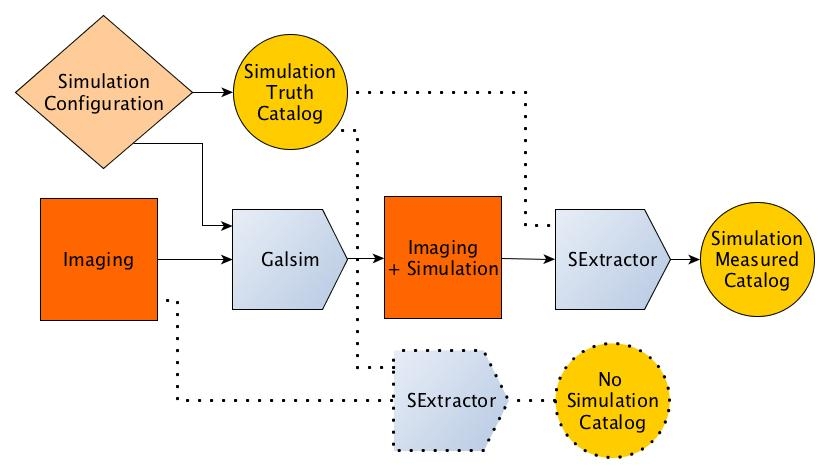
\includegraphics[width=0.9\linewidth]{flowchart.jpg}
\caption{Visualization of \balrog{}'s data flow. Optional (but also default) configurations are represented as dotted connections.}
\label{fig:flowchart}
\end{figure}

The \balrog{}  pipeline begins by opening a log file and parsing the command line parameters.
The code enforces a number of rules on the user's configurations.
If any errors or warnings occur they are directed to the log file. 
Errors are raised when users make a syntax error and \balrog{} cannot continue.
Generally, warnings occur when something is missing, but the code is able to continue using an internal default. 
Warnings likely, but not always indicate something is not quite right.
The log file remains open, recording messages through the full pipeline.

Next \balrog{} interprets how the user wants to generate their simulated galaxies.
\autoref{sec:galsim} fully prescribes the attributes of these galaxies.
To summarize, each galaxy is composed of one or more \sersic{} profiles.
The user's directives are executed, and  a truth catalog of the galaxy parameters is written.

The code then reads in the imaging data into which the simulated galaxies will be drawn.
Refer to \autoref{sec:data} to define what is required of the imaging data in this context.
By default, \sex{} is run over the input image. Please note, at this point no simulated
galaxies have been inserted. However, this command is potentially useful
for reasons discussed further in \autoref{sec:processing}.
An image of each galaxy, commonly known as a postage stamp, is generated and then added atop the input image.
Galaxy postage stamp drawing is treated in \autoref{sec:galsim}.
Once galaxies have been added to the image, \sex{} is called again.
Details of \sex{}'s implementation are deferred to \autoref{sec:processing}.
\sex{} outputs a catalog of the object measurements, which is now ready
for the user to compare with the trutch catalog.


\section{Input Data}
\label{sec:data}

\balrog{} reads in an astronomical image of pixellated flux values.
The data should include a photometric calibration defining
what one ADU count means physically. 
Galaxy simulations are done in apparent magnitude space,
and \balrog{} needs a zeropoint, $m_z$, to convert this to an image ADU level.
$m_z$ is defined in the usual way, where the objects flux, $\mathcal{F}$,
and apparent magnitude, $m$, are related by:
$m - m_ z = -2.5 \log_{10}(\mathcal{F})$.
A default zeropoint of 30 is assumed if one is not otherwise specified.
Required with each image is the image's weight map and PSF model. 
The weight map will be needed when extracting the sources from the image.
At a minimum, the PSF model is necessary for convolving the simulated galaxies
prior to  embedding them in the given image.
It is also obligatory if attempting to fit models to deconvolved measurements of galaxy profiles
during the source measurement process.
The only file type \balrog{} supports for input PSF models is that generated by 
\psfex{}\footnote{\url{www.astromatic.net/software/psfex}} \citep{psfex}.
Readers should be aware that \balrog{} itself does not run \psfex{}.
Thus, generating \psfex{} models constitues a prerequisite users must complete prior to running \balrog{}.
\balrog{} simulations incorporate \galsim{}'s WCS features, and hence
the software requires each image contain a WCS solution. \balrog{} reads this solution from the image's header.
If no WCS exists in the header, the pipeline enforces a fiducial WCS with a constant pixel scale of 
0.263~arcsec/pixel.\footnote{0.263~arcsec/pixel is the fiducial pixel scale for DECam.}
\balrog{} supports subsampling the input images if desired, meaning galaxies will only be
inserted into a portion of the image.
Once galaxies are simulated, the input image's flux values change by adding the galaxies fluxes to the original fluxes. 
Algorithmically, this is the only change applied to the input by the entire \balrog{} pipeline.
The weight map and PSF remain unchanged.
Conceptually, the bulk of the undertaking goes into simulationg the galaxies.

\hl{Is it worth adding some kind of support to generate the PSF model? This introduces some issues doing so, but it might be worthwhile.}

\section{Simulated Galaxies}
\label{sec:galsim}

To simulate galaxies, \balrog{} makes use of \galsim{}. 
It calls \galsim{}'s class for implementing \sersic{} objects to model the galaxies' light distriubtions as \sersic{} profiles. 
By effectively adding together these \sersic{} objects, \balrog{} allows galaxies to be composed of as many superimposed
\sersic{} components as desired. Each of these components has its own \sersic{} index, half light radius, flux,
minor to major axis ratio, and orientation angle. The half light radius is measured along
the major axis, and the orienation angle is measured as the major axis' counter-clockwise rotation
away from the $\hat{x}$-direction. 
Flux values are generated as magnitudes, then converted to ADU levels 
using the image's zeropoint.
In addtion to its \sersic{} components, each galaxy
shares five parameters which are identical among each \sersic{} component:
two centroid coordinate positions $(x, y)$, two components of reduced shear $(g_1, g_2)$, and magnfication.
The reduced shear follows the usual lensing notation convention, with positive $g_1$ along the $x$-axis,
negative $g_1$ along the $y$-axis, and positive and negative $g_2$ rotated 45\degree{} from the
respective $g_1$ counterparts. Magnification is the usual $\mu = 1 + \kappa$.
To be explictly clear, the shear and magnification are lensing effects applied to a galaxy,
and the axis ratio and orientation angle are intrinsic to the galaxy, as they would be in the abscence of lensing.

\balrog{} presents users with a number of different options for how to generate
the truth properties of their galaxies.
Simple types include a constant to be applied commonly to every galaxy or an array containing an element for each galaxy.
Alternatively, values can be sampled from the columns in a catalog file. 
Multiple columns from the same table are automatically jointly sampled.
Last but certainly not least, users can define their own functions which determine the truth paramters of the simulated galaxies.
This is perhaps \balrog{}'s most powerful feature.
It is this functionality which adds the flexibility for \balrog{} to support
virtually anything users can think of and code up in \py{} themselves.
Conveniently, the functions may operate over the galaxies' truth parameters themselves,
allowing one parmeter to be defined in terms of another.
\hl{Maybe I should say something along the lines that Catalog is quite useful if it reproduces the same distributions.}

The simulation process runs in a loop with a number of iterations equal to the number of galaxies to be simulated.
A subloop then iterates over the number of \sersic{} profiles the galaxies are composed of.
For each profile, a \sersic{} object is obstantiated with the \sersic{} index,
half light radius, and flux which were generated. Initially these objects are circularly symmetric
so the shearing method is called to create the galaxy's axis ratio, oriented in the appropriate direction.
All these elliptical objects inside the subloop are added together to create the composite galaxy made
of superimposed profiles. Lensing is then applied to the combined object, implementing both the
lensing reduced shear and magnfication.
The PSF model is sampled at the galaxy's centroid position and convolved with the galaxy profile.
Finally, the object is convolved with a top-hat pixel response function
whose scale is equal to that of the local WCS pixel scale.
\hl{Should I say something about how the PSFEx model is not automatically centroided and I have to do it in the code?}

The galaxy object is then drawn into a postage stamp image. 
The implemented drawing routine requires FFTs, whose targeted accuracies can be adjusted by users.
The pixel scale of the postage stamp is fixed to have the scale of the local WCS at the galaxy's position.
The size of the postage stamp is computed automatically by \galsim{} by dictating that
only a certain small enough fraction of the galaxy's flux is permitted to be lost outside the postage stamp's boundaries.
Noise is added to the galaxy's postage stamp by \galsim{}'s functions  for creating CCD-like noise.
The functionality relies on specifying the gain to set the noise level. 
This gain defaults to unity when nothing else if available.
\balrog{} sets the read noise to zero.
The final step in the simulation process is to add the postage stamp to input image, centering the
postage stamp onto the galaxy's generated $(x, y)$ centroid coordinates.


\section{\sex{} Implementation}
\label{sec:processing}


The default behavior is to run \sex{} in \emph{association mode}.
For those unfamilar with the terminology, association mode means
\sex{} will only make possible measurements at a predefined list of coordinates.
Here, the list is given as the simulated galaxies' locations. 
Hence, \sex{} is effectively aware of where in the image the simulated galaxies live.
If it finds an object at one of the these coordinates, it extracts it;
but it does not extract objects anywhere else.
This bypasses the need to extract every single object in the image. 
Namely, it  selects against the objects unrelated to the simulated galaxies that 
existed in the image prior to any simulation,
which have no truth information to compare with anyway.
The attractiveness of running in association mode is the reduction in execution time it offers.
In order to avoid simulated galaxies overlapping each other, simulated galaxies should be inserted
into the image at a significantly lower number density than the number density of the image itself.
This means association mode would suppress measurments for the majority of all objects.
By default \balrog{} configures \sex{} to make a \sersic{} fit to each simulated galaxy.
Because model fitting is a time expensive step,
association mode offers a significant payoff when using this configuration.
For a large dataset, running \sex{} many times over many images, model fitting 
each object in every run is likely time infeasible.

In addition to running \sex{} over the image with the simulated galaxies,
by default \balrog{} is configured to run \sex{} over the image prior to inserting the simulated galaxies.
This is to confirm if the association mode functionality of \sex{} is genuinely measuring a simulated galaxy.
For example, \balrog{} may happen to place a galaxy into the image at a location where a big, bright object already lives.
If the simulated galaxy is rather faint, \sex{} may just interpret its flux as part of the original object, having no
idea the simulated galaxy is even there. The \sex{} run over the pre-simulation image allows users to check
for such occurences if they would like. By default, this run does not include model fitting.
For the case described here, there is no benefit to dedicate the additional time needed for model fitting.


\chapter{What Is \balrog{} Good For?}
\label{sec:motivation}

No astronomical imaging survey is perfectly homogenous. Variations in
image quality and depth are a necessary result from any multi-epoch
measurement, even without variations in weather, sky brightness, or
telescope properties that can drive inhomogeneities within a single
epoch [REF: e.g. Holmes, Hogg, \& Rix 2012]. Effective use of imaging
data requires a good model for what happens to the data during
processing, but the process of creating a catalog from an image
generally is generally nonlinear\footnote{Thresholding does this, and
  no matter what else you do, all catalog-making requires
  thresholding.}, and the actual relationship between the resulting
data products and the world of forms can be quite difficult to model
analytically or even heuristically [e.g., SDSS sky subtraction, see
REF:Aihara paper, or any deblending algorithm ever].

Quantatively, what's missing is the likelihood function:
\begin{equation}
L = p( {\rm Catalog} | {\rm world\: of\: forms})
\end{equation}.
for a given data reduction and catalog-making recipe. This would be
necessary for a fully Bayesian imaging analysis (which is probably presently impractical
for any large imaging survey), but even for a catalog of
point estimates of object properties, $L$ is necessary to characterize
the noise and bias of the estimators.

We provide three examples of contemporary relevance below. For each of
these, we provide example pseudocode that shows how to compute the
quantity of interest using \balrog{}.

\section{Completeness}
The most common first step in any procedure (REF: SExtractor, PHOTO, maybe THELI?) for
creating a catalog from an image is a matched filtering of the image
followed by a thresholding. Typically, the filter is chosen to be
similar (in the broadest sense of similarity) to the expected image
psf [REF: Photo-lite, SEXtractor, etc.]. The resulting detection map
is thresholded, and the pixels that exceed the threshold become the
focus of subsequent analysis.

For a surface-brightness profile of the same shape as the filter, the
matched filter corresponds to the optimal\footnote{Really optimal, in
  the sense that it saturates the Cramer-Rao bound, and so a
  lower-variance unbiased estimator is mathematically impossible.}
measurement of the flux of an object at that position, so thresholding
the detection map corresponds to an actual flux limit. For other
surface-brightness profiles, however, this is not true, and any
catalog-making process that begins with this step cannot be said to be
``magnitude-limited'' or ``flux-limited''. This is a problem, because
the completeness of most astronomical imaging is very frequently
characterized by a single number, corresponding to the magnitude of
the faintest object in the catalog; occasionally, conscientious
authors will note a significance level (corresponding to the
threshold) or that the quoted limiting magnitude is appropriate
for either point-sources or galaxies. 

The most secure way to deal with this problem is to compute the
probability of detection for the ensemble of sources that will be
subjected to analysis. \balrog{} makes this step straightforward: by
embedding a catalog of objects in the real images, and then re-running
the catalog-making pipeline, it is easy to then determine, by
sampling, the detection probability for any objects of interest as a
function of their underlying properties.


\section{Clustering}
TODO: Detection probability as it varies across the sky, its effects
on correlation functions, and how to use \balrog{} to find this out.

\section{Optimization}
TODO: Demonstrate what you can do if you know the measurement
covariance matrix.



\chapter{Installation}
\label{sec:install}

\balrog{} consists of two depencies: \galsim{} and \sex{}.
\balrog{} itself is written entirely in \py{} and will run out of the box if  
\emph{sufficiently recent} versions of \galsim{} and \sex{} have already been installed.
As of the writing of this documentation,\footnote{\label{foot:date}\ericdate} 
\balrog{} requires the latest version of \galsim{}, which is version \codett{1.1}.
We have not thoroughly tested what constitues a \emph{recent enough} version of \sex{}.
What we are able to say is that the oldest version we have successfully tested against is \codett{2.17.0}.
\balrog{} and \galsim{} both exist as repositories on GitHub and can be downloaded 
from the command line.

\begin{cmdline}
% git clone https://github.com/emhuff/Balrog.git
% git clone https://github.com/GalSim-developers/GalSim.git
\end{cmdline}

\noindent This should automatically check out the master branch of each.
Master is the only supported branch for \balrog{}. 
The master branch of \galsim{} will always be a version $\geq$ \codett{1.1}.
\sex{} is packaged as a tarball, which can be downloaded 
from its \href{https://www.astromatic.net/software/sextractor}{official website}.
We recommend choosing the most recent version.

The \galsim{} documentation includes an extensive
\href{https://github.com/GalSim-developers/GalSim/blob/releases/1.0/INSTALL.md}{installation guide},
with many helpful hints and links to \codett{FAQ} pages. 
We refer \balrog{} users to this guide for how to install \galsim{}.
The \galsim{} team deserves a big thanks for the utility of their installation notes.
The \balrog{} authors are far from accomplished system adminstrators, 
but we both were independently successful installing \galsim{} on our systems by following these notes.

Section 3 of the \href{https://www.astromatic.net/pubsvn/software/sextractor/trunk/doc/sextractor.pdf}{\sex{} user manual}
contains a brief section explaining how to install the software. The code itself also includes a file called \codett{INSTALL}, with
slightly more detailed installation instructions.
One item not explictly stated in the installation notes is that \sex{} requires the ATLAS\footnote{\url{http://math-atlas.sourceforge.net/}}
linear algebra package as a dependency.
\sex{} will not install properly unless ATLAS is installed. 
The ATLAS website includes the requisite source code and
an extensive \href{http://math-atlas.sourceforge.net/atlas_install/}{installation guide}.
Once ATLAS builds and installs, the \sex{} installation steps should be straightforward to follow and complete.

To test the \balrog{} installation, change directories to the directory \codett{git} cloned for \balrog{}.
The directory contains a file called \codett{./balrog.py}. Run the file from the command line:

\begin{cmdline}
% ./balrog.py --fulltraceback
\end{cmdline}

\noindent If installation was successful, this will run without printing any error messages.

\chapter{Quick Start}
\label{sec:quick}

\balrog{} has been designed with flexibility of use in mind. As a necessary consequence, 
a number of different configuration possiblities exist, each of which must be
adequately explained, which quickly expands the length of the documentation.
We realize parsing the entirity of this manual requires some time.
Hence, the intent of the this section is to offer a short primer for a few of the most import features
\balrog{} users will want to become familiar with.
The comprehensive usage instructions are saved for later sections.
We will refer readers to the relevant comprehensive sections for more details.
Included in our startup guide is a brief aside specific to \sex{}.
Accoringly, we divide the section into two pieces:
\autoref{sec:quickbalrog} considers \balrog{} in general,
and \autoref{sec:quicksex} narrorws the focus \sex{} alone.


\section{\balrog{} Basics}
\label{sec:quickbalrog}

Throughout the current section, we will supplement the discourse with concrete example calls users can run.
In order to enable copying and pasting the commands into the user's terminal and running them verbatim,
users should create an alias to the \balrog{} excutable \py{} file, \codett{balrog.py}. 
This file is found in the directory which was pulled from GitHub during installation,
which we will refer to as \codett{\$INSTALLDIR} for convenience.
Adopting this convention, the alias statment looks as follows:

\begin{cmdline}
% alias runbalrog=`$INSTALLDIR/balrog.py'
\end{cmdline}

\noindent For convenient reference in later sections, we have effectively 
abbreviated what we have just defined in \autoref{tab:def}.

The fastest way to get started understanding how to configure and use \balrog{} is to
run it using the example files which come packaged with the software, and then examine the input
and output of the run. 
\balrog{} has been set up such that when the executable \py{}
file is called without any command line arguments, it will run over
the example files, filling in defaults as necessary. 
Thus, this initial call is as simple as:

\begin{cmdline}
?\bcmd{}?
\end{cmdline}

\noindent The rest of the examples here build off this call by adding additional configurations via command line arguments.
To explore the command line arguments, one can run the following command to print a useful summary:

\begin{cmdline}
?\bcmd{}? --help
\end{cmdline}

\noindent For more extended help, the command line arguments built-in to \balrog{} are detailed further in \autoref{sec:cmdline}.
In brief, they are used to specify input images and their properties, as well as configuration
files to use with \sex{}, and a few other variables every \balrog{} run will need to define. 
Each comes with a default \balrog{} will assume if the user does not supply one.
The default example's image data (\opt{image}), 
weight map (\opt{weight}), 
and PSF (\opt{psfin})
live in {\ttfamily \$INSTALLDIR/default\_example/}.
The \sex{} configuration files live in 
{\ttfamily \$INSTALLDIR/astro\_config/}. 
File names are intended to be reasonably transparent.
\balrog{} can be told to print messages more verbosely, 
and it is also instructive to repeat the example \balrog{} call in verbose mode.

\begin{cmdline}
?\bcmd{}? --stdverbosity v
\end{cmdline}

\noindent While the original call ran without printing anything, this one will write out some messages
relevant to \balrog{} filling in defaults for parameters.
Such messages can be helpful for users to recognize 
if they are not in fact using the files they think they are using.
Closely related to \opt{stdverbosity} is \opt{logverbosity}.
While \opt{stdverbosity} is for \codett{stdout}/\codett{stderr},
\opt{logverbosity} dictates the level of messaging logged to file.
Run the the previous command, but now flag the logging to verbose:

\begin{cmdline}
?\bcmd? --stdverbosity v --logverbosity v
\end{cmdline}

\noindent Opening the file found in \codett{\$INSTALLDIR/default\_example/output/balrog\_log/run.log.txt}
should contain exactly the same statements printed to the command line.
Saving output to file is useful when attempting to debug runs after-the-fact.
%Some debugging hints are offered in \autoref{sec:debug}.
Had any \balrog{} runtime errors occurred during the run,
\codett{run.log.txt} is the file they would be logged to.
Additionally, \balrog{} logs the exact value of each command line argument  in \codett{args.log.txt}
and directs all \sex{}'s \codett{stdout} to \codett{sex.log.txt}.

\begin{table}
\caption{Definitions used throughout this manual.}
\label{tab:def}
\begin{tabular}{l l}
\toprule \toprule
\textbf{Name} & \textbf{Meaning} \\ \midrule
\codett{\$INSTALLDIR} & Directory \codett{git} clones for \balrog{}, i.e. where \balrog{} is installed \\
\codett{runbalrog} & \codett{\$INSTALLDIR/balrog.py} \\ \bottomrule \bottomrule
\end{tabular}
\end{table}

The command line arguments attempt to be rather intuitive as to what they mean,
but one which may not be so obvious is \opt{pyconfig}.
In order to flexibly handle how galaxies will be simulated, \balrog{} accepts defined blocks of \py{} code
within the file specified by \opt{pyconfig}.
Owing to its command line name, we will refer to this file simply as the \pyconfig{} file
throughout the documentation.
Included within the \pyconfig{} file is support for implementing custom functions 
and command line arguments to be called upon during the galaxy generation process.
The core functions defined in \pyconfig{} files have a strictly
structured syntax which will be fully described in \autoref{sec:pyconfig}. 
The syntax is designed to be as natively \py esque as possible, so
many users will likely be able to extrapolate directly from examples without reading lengthy documentation. 
In the current \codett{runbalrog} examples, \opt{pyconfig} defaults to \codett{\$INSTALLDIR/config.py}.
This file builds galaxies as single component \sersic{} objects.
As an instructive guide, the file includes descriptive comment lines explaining what the different functions are used to do.
Rather than copying the comments into this document, we encourge user to open the \pyconfig{} file themselves.
Reading through the file itself is a more efficient method to quickly get started than
reading through anything else we could write here.
A slightly more sophisticated \pyconfig{} file can be found in \codett{\$INSTALLDIR/config2.py}.
This generates galaxies with both a bulge and a disk component.
Together, these two examples are designed to demonstrate the range of statements available to 
\balrog{}'s \pyconfig{} file.

All \balrog{} output is saved in subdirectories under the directory chosen by command line argument \opt{outdir}.
This directory has defaulted to \codett{\$INSTALLDIR/default\_example/output} for the example run.
The complete set of output generated by \balrog{} is detailed in \autoref{sec:out}.
In brief there are four subdirectories:
\codett{balrog\_log}, \codett{balrog\_image}, \codett{balrog\_cat}, and \codett{balrog\_sexconfig}.
We have already noted three log files written to \codett{balrog\_log}. In addition, an explicit copy of 
the user's \pyconfig{} file is also written there.
\codett{balrog\_image} includes a copy of any image \balrog{} either used or generated.
Ones with \codett{.sim} in their file names include the simulated galaxies, and ones with \codett{.nosim} do not.
\codett{balrog\_cat} contains \codett{example.truthcat.sim.fits}, the truth parameters assigned to simulated galaxies,
as well as the \sex{} catalogs \balrog{} generates.
Again, files including the simulated galaxies contain a \codett{.sim} in their names.
and the ones containing a \codett{.nosim} do not.
\codett{balrog\_sexconfig} copies the files \balrog{} used for configuring \sex{}.
When running \balrog{} over files other than the defaults, 
the output file names are automatically generated based on the input file names.
It may seem that a single run produces a substantial amount of output, but the idea
is that any \balrog{} call be reproducible and debuggable from its output in case anything does go wrong.

\section{\sex{} Basics}
\label{sec:quicksex}

Here, we momentarily center the attention soley on \sex{}.
However, before proceeding further, 
please take note that this treatment is not intended to be a comprehensive guide 
to running or understanding \sex{}.
Rather, we simply offer a few comments which will hopefully help run \sex{} successfully within \balrog{}.
For those who have never used \sex{}, we direct you to the
\href{https://www.astromatic.net/pubsvn/software/sextractor/trunk/doc/sextractor.pdf}{official \sex{} user manual} 
or alternatively the so-called
\href{http://astroa.physics.metu.edu.tr/MANUALS/sextractor/Guide2source\_extractor.pdf}{Source Extractor for Dummies} text.

\sex{} runs are configured via roughly a handful of files. 
In this scope, the two most relevant ones are given by command line arguments \opt{sexconfig}
and \opt{sexparam}. 
\codett{sexparam} files are often denoted with a \codett{.param} extension in their file names,
while \codett{sexconfig} files are often denoted with a \codett{.sex} extension in their file names.
In the example files shipped with \balrog{}, the \codett{sexconfig}
file is suffixed with a \codett{.config} extension for consistency with our terminology.
\codett{sexconfig} is allowed to specify any of the arguments which can
also be given as command line arguments to \sex{}.
These set conditions such as the detection thresholds,
the aperture sizes for photometry, the magnitude zeropoint,
and the background subtraction strategy.
The \codett{sexparam} file is a list of keywords.
Each keyword is a measurment \sex{} will make for every extracted object, which will therefore
appear as a column in the output catalog.

It is \codett{sexparam} which controls whether or not \sex{} will perform model fits to the galaxies. 
How do to this is rather scarely documented, but has been passed down by word of mouth in the Astronomy community. 
We consider it worthwhile to elaborate in writing.
\sex{} includes up to two possible types of models to fit.
One, denoted by the key \codett{DISK}, is a model with fixed \sersic{} index of $n=1$,
i.e. an exponential.
The other, denoted by the key \codett{SPHEROID}, is a model with a free \sersic{} index.
\sex{} can fit either of these independently or both simultaneously.
Each model written into and uncommented from the \codett{sexparam} file is fit,
meaning if just the \codett{DISK} key is present a disk only model with $n=1$ is fit;
if just the \codett{SPHEROID} key is present a bulge only model with free $n$ is fit;
and if both \codett{DISK} and \codett{SPHEROID} keys are present both the
disk and bulge are fit simultaneously, which is of course different than fitting them independently.
Each model can fit for the flux, magnitude, axis ratio, and orientation angle of the model.
The spheroid model also fits the sersic index and half light radius.
The disk model fits the scale radius, as opposed to the half light radius.
Open the \codett{bulge+disk.param} file included with \balrog{} in the \codett{astro\_config} directory
for the \sex{} names of all the parameters.
The meanings of the \codett{DISK} and \codett{SPHEROID} names are human understandable.


\chapter{Native Command Line Arguments}
\label{sec:cmdline}

\balrog{} runs can be configured via command line arguments.
Two categories of arguments exist. 
First are the built-in ones, native to \balrog{}.
These constitute the focus of this section.
In addition, \balrog{} also supports a mechanism for users to define their own command line arguments.
However, because the functionality is drawn from what we have deemed the \pyconfig{} file,
its treatment is saved for \autoref{sec:user}.
To generate a summary of \balrog{}'s command line environment, run the following command,
where \codett{runbalrog} is defined in \autoref{tab:def}.

\begin{cmdline}
?\bcmd? --help
\end{cmdline}
This prints a listing of all the command line arguments (including those defined by the user), 
along with their available help strings.
The built-in arguments' help strings are intended to be a useful quick reference tool,
but in order to preserve suitable readability from the command line, 
they do not necessarily spell out every possible detail users may wish to know.
Accordingly, we include a more extensive supplement within this section.

We direct the reader's attention to \autoref{tab:opts}.
It is a comprehensive listing, containing an entry for each of \balrog{}'s command line arguments.
\autoref{tab:opts} is the core substance of this section,
and is intended to be more or less readable on it own, apart from the text of the document.
Ergo, we refrain from copying every detail from \autoref{tab:opts} into the text, 
preferring the orderly organization and conceptual clarity
of the table over something which would require many more words to describe in paragraph form.
However, we will make a few general comments to put \autoref{tab:opts} into better context.

Each command line argument can be specified either with its full name or an abbreviated form, e.g. \opt{imagein} vs. \opt{ii}.
The full names attempt to be as intuitive as possible while maintaining a reasonbly small number of characters.
The abbreviatons trade clarity for brevity for those who prefer compactness. 
Any parameter that  is left out of a user's \balrog{} call assumes a default value in the code.
Each of these defaults is listed in \autoref{tab:opts}. 
In a few cases, the default values are conditionally defined, meaning \balrog{} will select one out of
two possible defaults depending on how the run has been configured.
\autoref{tab:opts} utilizes pseudocode to explain the behavior of how these defaults are ultimately chosen.
When \balrog{} parses the user's command line, it performs a number of checks, 
thereby enforcing proper data types, file existence, etc.
Warnings or errors are raised as needed.
\autoref{tab:opts} has been grouped into subcategories of similar parameters.
The divisions do not matter per se; they are merely an organizational guide.
However, because \balrog{} contains quite a few possible arguments to adjust,
we find them to be a useful aid in adding to tractability.

\opt{sexconfig} and \opt{sexparam}/\opt{sexemptyparam} require a bit more explanation than is practical
within the space of \autoref{tab:opts}
First, not every keyword-value pair in \opt{sexconfig} is relevant during \balrog{} runs.
Please note, we are not trying to say these settings have zero or very little effect on \sex{}.
What we mean is that their values within \opt{sexconfig} will be ignored by \balrog{}, because
the values are deduced directly from \balrog{}'s command line, and then 
given as \sex{} command line arguments, which override the \codett{sexconfig} file.
These amount to what has been written into \autoref{tab:b2s}.
\autoref{tab:b2s} notes that the \opt{sexconfig} and \opt{sexparam}/\opt{sexemptyparam} given to \balrog{}
are not necessarily exactly the ones used when running \sex{}.
This is to account for the syntax differnce between running with association mode on or off.
If association mode is on, a \codett{sexparam} file must be written with the proper \codett{VECTOR\_ASSOC} line.
\balrog{} does so, and then uses the file. Settings in \codett{sexparam} files cannot be overridden from \sex{}'s command line.
If association mode is turned off \balrog{} must make sure that no \codett{ASSOC\_*} keywords exist in the \codett{sexconfig} file,
and writes one out where this is the case for usage downstream. To the best of the authors' knowledge,
settings like \codett{ASSOC\_*} present in a \codett{sexconfig} file cannot be removed entirely via command line overriding.
Striclty speaking, there is not a problem if \codett{VECTOR\_ASSOC} is present in the \codett{sexparam} file with association
mode off, but \balrog{} will write and use ones assuredly without it in order to avoid unnecessary warnings.
We emphasize, no loss generality has been lost for running \sex{}.
We have just automated the process of creating an on/off switch for association mode, and moved some
configurations to \balrog{}'s command line because other \balrog{} functionality besides \sex{} depends on them as well.
At any rate, \balrog{}'s output logs will allow users to read off exactly how their \sex{} commands were called (c.f. \autoref{sec:out}).

\newpage
\optstab{}

\begin{table}[h]
\caption{Translation between \balrog{} command line argument names and \sex{} command line argument names.} \label{tab:b2s}
\begin{tabular}{l l l} \toprule \toprule

\textbf{\balrog{}} & & \textbf{\sex{}} \\ \midrule \\
\multicolumn{2}{c}{\dfill} & Explit \hspace{0.3cm} \dfill \\
\opt{imagein} & $\rightarrow$ & \codett{IMAGE} \\
\opt{weightin} &  $\rightarrow$ & \codett{WEIGHT\_IMAGE}\\
\opt{sexnnw} & $\rightarrow$ & \codett{STARNNW\_NAME} \\
\opt{sexconv} & $\rightarrow$ & \codett{FILTER\_NAME} \\
\opt{zeropoint} & $\rightarrow$ & \codett{MAG\_ZEROPOINT} \\
\opt{psfin} & $\rightarrow$ & \codett{PSF\_NAME} \\
\opt{catfitstype} & $\rightarrow$ & \codett{CATALOG\_TYPE} \\
\opt{outdir} & $\rightarrow$ & \codett{CATALOG\_NAME} \\ \\

\multicolumn{3}{c}{\dfill - - - - Possibly Modified To Account For Association Mode - - - - \dfill} \\
\opt{sexconfig} & $\rightarrow$  &\codett{c} \\
\opt{sexparam}/ & $\rightarrow$  &\codett{PARAMETERS\_NAME} \\ 
\opt{sexemptyparam} & \\ \\ \bottomrule \bottomrule
\end{tabular}
\end{table}


\chapter{\balrog{}'s \texttt{pyconfig} File}
\label{sec:pyconfig}

As introduced in previous sections, \balrog{}'s \pyconfig{} file is a configuration file for \balrog{} made up of \py{} statements.
Relying on the ease and simplicity of writing \py{} code, this file is what contributes a large portion of \balrog{}'s flexibility.
The authors cannot natviely build-in to \balrog{} all the features every user would like to see.
Thus, we attempt to create an enviroment which makes it easy for users to fold in additional content themselves.
The \pyconfig{} file plays a significant role in \balrog{}, and hence we will take care to provide adequate documentation.

As far as general comments go, we remark that the \pyconfig{} file makes use of five core functions called:
\argsfunc, \parsefunc, \simfunc,  \gspfunc, and \sexfunc.
\balrog{} checks for functions of exactly these names.
If one of the function does not exist,
\balrog{} continues by skipping the portion of the code where the function would have been called.
An omission should not cause the \balrog{} run to fail; however, some level of flexibility will have been lost.
We issue warning messages to alert the user when one or more of the functions are missing.

Each of the five core functions in \pyconfig{} will be described further in what follows.
However, it is also important to keep in mind their overall workflow on a more conceptual level.
Algorithmically, what occurs is users create command line arguments then parse them appropriately.
These arguments, as well as the one \balrog{} relies on natively, are then made available to 
functions which implement \py{} statments to define how \balrog{}'s galaxies are simulated.
We have included some convenience features to coordinate the coding of the simulation specfications,
including support for users to write their own functions to do so.
Within the \pyconfig{} environment, it is also possible to override some \sex{} configurations if desired,
implementing a certain level of \py{} control of \sex{}.

In the remainder of \autoref{sec:pyconfig} we concentrate on \pyconfig{}'s usage, with a particular focus on elucidating its syntax.
\autoref{sec:user} treats user-defined command line arguments within \pyconfig{} and 
\autoref{sec:simrules} illustrates how \pyconfig{} specifies simulated galaxy generation.
\autoref{sec:sexoverride} describes the way in which \pyconfig{} can be used to override \sex{} settings in \opt{sexconfig}.
As an aid while reading this section, 
we strongly encourage users to open one of the example \pyconfig{} files shipped with \balrog{},
\codett{\$INSTALLDIR/config.py} or \codett{\$INSTALLDIR/config2.py}.
As mentioned in \autoref{tab:def}, \codett{\$INSTALLDIR} is the directory where \balrog{} is installed.

\section{User-Defined Command Line Environment}
\label{sec:user}

Within the \pyconfig{} file, the definitions for custom command line arguments occur inside the \argsfunc{} function.
Passed to \argsfunc{}  as a function argument is \argsparser{},
an object made by \codett{python}'s
\codett{argparse.ArgumentParser()}. Arguments
can be added to parser according to the usual
\codett{argparse} syntax.
For those unfamilar with \codett{argparse},
\href{http://docs.python.org/2/howto/argparse.html}{this tutorial}
contains many useful examples. A simple example of
\argsfunc{} is copied below.

\begin{code}
def CustomArgs(parser):
    parser.add_argument( "-cs", "--catalogsample", help="Catalog used to sample simulated galaxy parameter distriubtions from", type=str, default=None )
\end{code}

\noindent Users are allowed to add arguments by any names except those already defined as native \balrog{} command line arguments.
Adding two arguments of the same name in the \codett{ArgumentParser} class raises an exception.
The utility of adding custom command line arguments is that the values given to the arguments
are made available to the other core functions in \pyconfig{}.

The user-defined arguments are parsed within \parsefunc{}.
When this function is called, 
\balrog{} has already grabbed any of the user's custom arguments from the command line,
and saved them into an object called \parseargs{}.
\parseargs{} is passed as the single function argument to \parsefunc{}.
It is equivalent to an object returned by \codett{parser.parse\_args()};
each one of the user's command line arguments becomes an attribute of \parseargs{}. 
\parsefunc{} allows users to apply any \py{} operations they so desire to their arguments.
A simple version of \parsefunc{} has been included below:

\begin{code}
def CustomParseArgs(args):
    thisdir = os.path.dirname( os.path.realpath(__file__) )
    if args.catalogsample==None:
        args.catalogsample = os.path.join(thisdir, `cosmos.fits')
\end{code}

\noindent As the example demonstrates, one feature of the \parsefunc{} is a convenient
way for users to effectively define new defaults for \balrog{} using
commonly-known ordinary python syntax.
More generally, different \balrog{} runs are now capable of recognizing and appropriately parsing
completely different sets of input parameters. 

Returning to \parseargs{},
the object not only contains an attribute for each of the user's customly defined arguments,
its attributes also include each of the native \balrog{} arguments.
When \parsefunc{} is called, the built-in arguments have already been parsed,
so arguments which were left out of the command line call have assumed their defaults.
Inside \pyconfig{}, users are allowed to modify the attributes of \parseargs{} derived from bult-in \balrog{} arguments, 
if they so desire.
However, in order to prevent changes from potentially causing unhandled exceptions later in \balrog{},
any modifications will not propogate outside the \pyconfig{} file.
\balrog{}'s native arguments will behave according to how they were specified at the command line.
Thus, allowing changes to the native attributes is more of a local convenience than anything else.

\parseargs{} will be given as a function argument to the \simfunc{}, \gspfunc, and \sexfunc{} functions.
Changes within these functions to \parseargs{}'s attributes, both those derived from native or custom arguments,
are also effectively \emph{local only}.
Modifications made in one of the functions do not propogate outside that function.
The code has been written this way so users do not need to consider the order in which the three functions execute
in order to know excatly what \parseargs{} they are using in each function.
The behavior is consistent with including the \parsefunc{} in the first place.
The only place to make persisting changes to \parseargs{} is \parsefunc{}.
\hl{I need to incorporate the new args behavior into the code.}

Please note, no parsing of any kind can be done inside \argsfunc{}.
\argsfunc{} is for definitions only.
It informs \balrog{} what it should be looking for when it receives a command line.
No values have yet been assigned to any of the defined parameters when \argsfunc{} exits.
\parsefunc{} on the other hand tells \balrog{} what do once it has actually recieved the command line
and has saved each of the parameters into an attribute of \parseargs{}.

\section{Defining How to Simulate Galaxies}
\label{sec:simrules}

Deciding how the simulated galaxy properties should be sampled occurs inside the function \simfunc{}.
Passed into the \simfunc{} are three arguments: \simargs{}, \simrules{}, and \simsamp{}.
As discussed in \autoref{sec:user},
\simargs{} refers to the parsed command line arguments, both native \balrog{} and user-defined.
\simrules{} is an object whose attributes are overwritten
in order to specify how simulated galaxies are sampled.
\simsamp{} gives access to simulated galaxy parameters
after they have been sampled. \simrules{} and \simsamp{}
will become clearer to follow.

\begin{table}
\caption{Attributes of the \simrules{} object defining the simulated galaxies.} \label{tab:attr}
\begin{tabular}{l l}
\toprule \toprule
\textbf{Attribute} & \textbf{Meaning} \\ \midrule
\rules{x} & Galaxy centroid $x$-coordinate [pixels], $x \in \left[1,N_{cols} \right]$\\
\rules{y} & Galaxy centroid $y$-coordinate [pixels], $y \in \left[1,N_{rows} \right]$\\
\rules{g1} & Reduced shear, $g_1$ component \\
\rules{g2} & Reduded shear, $g_2$ component \\
\rules{magnification} & Magnification, $1 + \kappa$ \\
\rules{sersicindex} & \sersic{} index \\
\rules{halflightradus} & \sersic{} half light radius [arcsec] \\
\rules{magnitude} & Galaxy brightness [mag] \\
\rules{axisratio} & Minor to major axis ratio \\
\rules{beta} & Orientaiton angle of major axis (measured from $x$-axis) [degrees] \\ \bottomrule \bottomrule
\end{tabular}
\end{table}

\autoref{sec:galsim} laid out the parameters which characterize each simulated galaxy.
Briefly recapitulating, each galaxy is made up of one or \sersic{} profiles.
Each \sersic{} profile is composed of five components: 
\sersic{} index ($n$), half light radius, brightness magnitude, minor to major axis ratio, 
and orientation angle counter-clockwise from the $\hat{x}$-direction ($\beta$).
Furthermore, a simulated galaxy also shares fives additional parameters among each \sersic{} profile:
two centroid position coordinates, $(x,y)$, two reduced shear coordinates $(g_1,g_2)$, and magnification.
This totals ten ``\emph{variables}'' which fully specify the galaxy.
\simrules{} and \simsamp{} are each composed of ten attributes,
matching these same ten variables.
The attribute names for \simrules{} and \simsamp{} have been transparently chosen.
Nevertheless, for completeness the names and meanings are fully specified in \autoref{tab:attr}.
\autoref{tab:attr} uses \simrules{} as the concrete example.
The attribute names of \simsamp{} are identical. 
For the time being, we will continue assuming each galaxy has been simulated as a single \sersic{} profile.
We will return to handling two or more in a few paragraphs.

\begin{table} 
\caption{Syntax examples for each of the simulation types \balrog{} understands.} \label{tab:simtype}
\begin{tabular} {l l}
\toprule \toprule
\textbf{Type} & \textbf{Example} \\ \midrule
Constant & \codett{rules.g1 = 0} \\
Array & \codett{rules.x =  np.linspace(args.xmin, args.xmax, args.ngal)} \\
(Sampled  & \codett{rules.y = sampled.x}) \\
Catalog & \codett{rules.magnitude = Catalog(file=`cosmos.fits', ext=1, col=`IMAG')} \\
Function & \codett{rules.y = Function(function=rand,} \\
 & \hspace{1.55in} \codett{args=[args.xmin,args.xmax,args.ngal])} \\ \bottomrule \bottomrule
\end{tabular}
\end{table}

Users overwrite
each of the \simrules{} object's attributes to define their simulations.
Assignments can assume four (or possibly five depending how categorized) types of statements. 
The syntax for each is designed to be straightforward, intuitive, and \py{}esque.
For quick reference, an example of each is included in \autoref{tab:simtype}.
The first type of rule assignment is a constant, meaning each of the galaxies in the simulated galaxy sample
will have the same value for the selected parameter, e.g. \codett{rules.g1 = 0}.
Second, rule types can also be given as an array, equal in length to the number of simulated galaxies. 
Simulated galaxy $i$ for the chosen parameter then assumes the value in element $i$ of the array.
The example in \autoref{tab:simtype} is given as \codett{rules.x =  np.linspace(args.xmin, args.xmax, args.ngal)},
meaning galaxies will be evenly spaced along the $x$-axis across the image.
The third sampling type for \simrules{} is drawing from a catalog. 
This makes use of a function \balrog{} has defined called \codett{Catalog}. 
Calls to \codett{Catalog} require three arguments: \codett{file}, \codett{ext}, and \codett{col}.
\codett{file} is the file path to a FITS file;
\codett{ext} identifies which extension contains the data table to use; and
\codett{col} is the name of the column to draw from.
If \codett{Catalog} is used multiple times,
multiple columns selected from the same data table are automatically jointly sampled.
An example call to \codett{Catalog} looks like: 
\codett{rules.magnitude = Catalog(file=`cosmos.fits', ext=1, col=`IMAG')}.
Last but not least, the fourth assignable sampling type to \simrules{} is a function. 
Users write their own function according to usual \py{} syntax,
then feed this function and its necessary arguments as the arguments to
\balrog{}'s \codett{Function} command. 
The one requirement of sampling functions is they must return an array equal in 
length to the number of simulated galaxies.
Like the array sampling type, galaxy $i$ will use element $i$ of the returned array as its truth parameter.
Here, we provide an example code snippet, illustrative of how one could place the simulated galaxies at random image positions. 

\begin{code}
def rand(minimum, maximum, ngal):
    return np.random.uniform( minimum, maximum, ngal )

def SimulationRules(args, rules, sampled):
    rules.x = Function(function=rand, args=[args.xmin, args.xmax, args.ngal])
    rules.y = Function(function=rand, args=[args.ymin, args.ymax, args.ngal])
\end{code}

\noindent \codett{Function} affords a great deal of flexiblity toward
simulating a wide variety of different scenarios.
We will make further statements regarding slightly more sophisticated usage
of \codett{Function}, but it is useful to consider a few other points first.

Let us now return to the \simsamp{} object which is passed to \simfunc{} as an argument.
\simsamp{} is used in conjuction with \simrules{} to define one parameter's rule in terms of another's.
Conceptually speaking, \simsamp{} can be thought of an object whose attributes are arrays that 
have been set equal to the simulated galaxy parameters post sampling.
One might consider \simsamp{} its own sampling type, but at the same time, its also functionally equivalent to an array.
This is why a Sampled type has been added as a fifth entry in \autoref{tab:simtype}, in parentheses directly under the Array line.
To better understand \simsamp{}, consider the following code sample:

\begin{code}
def SimulationRules(args, rules, sampled):
    rules.x = Function(function=rand, args=[args.xmin, args.xmax, args.ngal])
    rules.y = sampled.x
\end{code}

\noindent The $x$-coordinates randomly sample, and then each galaxy's $y$-coordinate
is set equal to exactly the same value as its $x$-coordinate.
Please note, this is expressly different from the original example where both $x$ and $y$ sampled randomly.
\simsamp{} can also be used as an argument within the \simargs{} passed to a sampling function,
as is the case in the proceeding example.

\begin{code}
def SimulationRules(args, rules, sampled):
    rules.x = Function(function=rand, args=[args.xmin, args.xmax, args.ngal])
    rules.y = Function(function=rand, args=[args.ymin, args.ymax, args.ngal])
    rules.axisratio = Function(function=SampleFunction, args=[sampled.x, sampled.y,args.xmax, args.ymax])

def SampleFunction(x, y, xmax, ymax):
    dist = np.sqrt(x*x + y*y)
    max = np.sqrt(xmax*xmax + ymax*ymax)
    return dist/max
\end{code}

\noindent This functionality allows users to have access to the sampled galaxy truth
information in their functions.
This particular example gave each galaxy a position dependent axis ratio.
As a further eample, one could apply position dependent lensing effects in a similar fashion.

Thus far we have been operating with single component \sersic{} models.
However, two or more components can be implemented.
Doing so requires a call to a \balrog{} function called \codett{InitialSersic}
before any of \codett{rules}'s five \sersic{} attributes 
(\codett{sersicindex}, \codett{halflightradius}, \codett{magnitude}, \codett{axisratio}, \codett{beta})
are reassigned.
\codett{InitialSersic} takes \simrules{} and \simsamp{} as arguments as well as \codett{nProfiles},
the number of superimposed \sersic{} models, e.g.\\
\codett{InitializeSersic(rules, sampled, nProfiles=2)}.
This has recast the \sersic{} components of \codett{rules} and \codett{sampled} as length two list.
Now the elements of these attributes of \codett{rules} must be updated accordingly,
using syntax akin to that of any other \py{} list. For example, the following builds
galaxies as bulge + disk models, using an exponentional disk ($n = 1$) and a de Vaucouleurs bulge ($n = 4$).

\begin{code}
def SimulationRules(args, rules, sampled):
    rules.x = Function(function=rand, args=[args.xmin, args.xmax, args.ngal])
    rules.y = Function(function=rand, args=[args.ymin, args.ymax, args.ngal])
    rules.g1 = 0
    rules.g2 = 0
    rules.magnfication = 1

    InitializeSersic(rules, sampled, nProfiles=2)
    rulex.sersicindex = [1, 4]
    rules.halflightradius[0] = Catalog(`cosmos.fits',1,`HALF_LIGHT_RADIUS')
    rules.halflightradius[1] = sampled.halflightradius[0]
    rules.magnitude[0] = Catalog(`cosmos.fits',1,`IMAG')
    rules.magnitude[1] = sampled.magnitude[0]
    rules.beta[0] = Function(function=rand, args=[-90, 90, args.ngal])
    rules.beta[1] = sampled.beta[0]
    rules.axisratio[1] = sampled.axisratio[0]
    rules.axisratio[0] = Function(function=rand, args=[0.05, 1, args.ngal])
\end{code}

\noindent The example uses bulges and disks with identical half light radii,
magnitudes, axis ratios, and orientation angles.
The values for the half light radius and magnitude are sampled from the catalog \codett{cosmos.fits}.
The axis ratios and orientations angles are random, as are the galaxy positions.
No lensing is applied.
We direct the reader's attention to the final two lines.
Conceptually one would often think of these in the opposite order, but either is permissible 
and equivalent in \balrog{}.
Also notice that the \codett{x}, \codett{y}, \codett{g1}, \codett{g2}, and \codett{magnification}
attributes are unaffected by the \codett{InitializeSersic} statement. These attributes are never lists.


All attributes of \simrules{} have a default, which will be used if the attribute is not overwritten.
Any time a default must be used a warning message is issued.
The defaults themselves are listed in \autoref{tab:default}.
Notice that in some cases, the default is to sample from the \codett{cosmos.fits} catalog which
ships with \balrog{}.
These should create realistic populations.
By default a single component \sersic{} model is adopted.
If the \sersic{} mode is multi-compoents, each element of an attribute's list assumes the default in \autoref{tab:default}.
Whenever one uses \codett{InitializeSersic}, the \sersic{} attributes 
are reinitialized to their defaults, so be careful if \codett{InitializeSersic} is called more than once
in \simfunc{}.

\begin{table}
\caption{\simrules{} defaults.
\hl{I need to change the defaults for axis ratio and beta.}}  \label{tab:default}
\begin{tabular}{l l} \toprule \toprule
\textbf{Attribute} & \textbf{Default} \\ \midrule
\rules{x} & \codett{np.random.uniform(args.xmin, args.xmax, args.ngal)} \\
\rules{y} & \codett{np.random.uniform(args.ymin, args.ymax, args.ngal)} \\
\rules{g1} & 0 \\
\rules{g2} & 0 \\
\rules{magnification} & 1 \\ \\
\catline{\sersic{}} \\ 
\multicolumn{2}{c}{(If \sersic{} attributes are multi-component, each list element uses  this default)} \\ \\
\rules{sersicindex} & \codett{Catalog(`cosmos.fits',1,`SERSIC_INDEX')} \\
\rules{halflightradius} & \codett{Catalog(`cosmos.fits',1,`HALF_LIGHT_RADIUS')} \\
\rules{magnitude} & \codett{Catalog(`cosmos.fits',1,`IMAG')} \\
\rules{axisratio} & 1 \\
\rules{beta} & 0 \\ \bottomrule \bottomrule
\end{tabular}
\end{table}

Previouly we mentioned we would elaborate further on some finer details of using \codett{Function} to sample.
We now do so.
Inside \codett{Function} statements, it is possible to make an element of \simargs{} a \codett{Catalog} statement.
Here is a concrete example.

\begin{code}
def SimulationRules(args, rules, sampled):
    nc = Catalog(file='cosmos.fits',ext=1,col='SERSIC_INDEX')
    n = Function(function=g, args=[1, 0.05, args.ngal, nc])
    rules.sersicindex = n

def g(avg, std, ngal, add):
    gaus = gaussian(avg, std, ngal)
    return gaus+add

def gaussian(avg, std, ngal):
    return np.random.normal( avg, std, ngal )
\end{code}

\noindent An amount which is sampled from the catalog is added to the Gaussian.
This particular implementation is merely illustrative, not necessarily
something one would realistically do scientifically.
If the table given in \codett{Catalog} was also used to sample any other parameters,
everything is still automatically jointly sampled.
\codett{Function} can also take other \codett{Function} statments as elements of \simargs{}.
To demonstrate, we form another example very similar to the previous one.

\begin{code}
def SimulationRules(args, rules, sampled):
    ns = Function(function=exact, args=[np.ones(args.ngal)])
    n = Function(function=g, args=[4, 0.05, args.ngal, ns])
    rules.sersicindex = n

def exact(item):
    return item

def g(avg, std, ngal, add):
    gaus = gaussian(avg, std, ngal)
    return gaus+add

def gaussian(avg, std, ngal):
    return np.random.normal( avg, std, ngal )
\end{code}

\noindent Here, the usage of the \codett{exact} funciton is trivial, but nevertheless
representive of the proper usage.

\simfunc{} is written to be handle errors.
When users try to enter a sampling specification that \balrog{} does not understand an exception is raised.
Exceptions are also raised if users attempt to reassign attributes of \simsamp{} or 
access an attribute of \simrules{} or \simsamp{} which does not actually exist.
The mentioned exceptions cause \balrog{} to terminate.
The logic is that any \balrog{} \pyconfig{} syntax errors are treated like ordinary \py{} syntax
errors and thus force the execution thread to exit.
The traceback will include line numbers for where the process was terminated.

The final consideration to make about generating simulated galaxies is the function \gspfunc{}.
This function is passed three arguments: \codett{args}, \codett{gsparams}, and \codett{galaxies}.
\codett{args} is the same parsed command line argument object as passed given to \simfunc{}.
Likewise, \codett{galaxies} is the same object as \codett{sampled}.
It has just been renamed for clarity.
\codett{gsparams} is an object which populates each galaxy's \galsim{} \codett{GSParams}.
\codett{gsparams} has an attribute for each \codett{GSParam}, 
and the attributes behave essentially the same as the non-\sersic{} components of \simrules{}.
Each attribute of \codett{gsparams} can take on the same four (five) sampling types as \simrules{}:
a constant, array, (\codett{galaxies} attribute--not particularly useful here on its own but could be
inside \codett{Function}), \codett{Catalog}, or \codett{Function},
where all the same functionality applies to \codett{Function} as above.

Understanding all the \codett{GSParams} is a fairly technical subject, so we
refer users who need to adjust them to 
\galsim{}'s \href{http://galsim-developers.github.io/GalSim/structgalsim\_1\_1\_g\_s\_params.html}{GSParams reference page}
for the complete details.
In the context of \balrog{} these parameters are relevant for drawing the galaxies into postage stamp images.
\codett{alias\_threshold}, for example, determines what maximum fraction of the galaxy's flux may be lost outside the boundaries
of the postage stamp when determining how large of a postage stamp is needed for drawing the galaxies.
Convolution with the PSF and pixel response function is done in Fourier Space.
\codett{maxk\_theshold} determines the maximum $k$ used in FFTs such that $k$-values must fall below \codett{maxk\_threshold}
before cutting off the FFT. We will mention, there are also parameters for setting target accuracies.
Each \codett{GSParam} has a built-in \galsim{} default. Any attribute not explictly
assigned in \gspfunc{} uses this default.
In most cases, the defaults work well enough. The exception is when very bright objects ($\sim$~15 mag, depending on the calibration)
are being drawn, and even a small percentage of the flux totals to a signifcant number of ADU.
If you think there might be an issue visually inspect the image into which the simulated galaxies have been drawn (c.f. \autoref{sec:out})
for signs of aliasing.

\hl{Do we want a table of these? I can easily get the defaults, but as far as I can find, they're not even
on the Galsim help page. Maybe make an appendix table? It doesn't really hurt putting them in, it just might
be a bit confusing/overwhelming to some people.}


\section{\sex{} Configuration Overrides}
\label{sec:sexoverride}

The final of the core functions in \pyconfig{} which we are yet to discuss in detail is \sexfunc{}.
This function is very simple. It is passed two arguments: \codett{args} and \codett{config}.
As was the case in \simfunc{} and \gspfunc{}, \codett{args} contains the parsed command line arguments.
\codett{config} is a dictionary. Users are free to add to the dictionary the keyword-value pairs
that a \codett{sexconfig} file understands. These will then override what was given in \opt{sexconfig}
by giving them as command line parameters to \sex{}.
This effectively allows users to do anything from the \balrog{} command line they could do from the \sex{} command line.
While none of the keywords will cause an error in \sexfunc{}, 
the same issue discussed in \autoref{sec:cmdline} applies here.
A dozen or so of the keywords will not actually overwrite anything.
Namely, each of the \sex{} parameters in the right-hand column of \autoref{tab:b2s} cannot explicitly be overridden via \codett{config}.
To ensure proper implementation of \sex{}'s association mode, no \codett{ASSOC\_*} keywords added to \codett{config}
would have any effect either.


\chapter{Output}
\label{sec:out}
Each \balrog{} run generates a number of output files. 
At first, this number may seem larger than was perhaps expected.
However, we air on the side of writing to disk anything users might possibly want afterward.
We intend for \balrog{} to be transparent and debuggable.
All runs should be recreateable from their output files.

The output files are organized into a fixed directory structure.
Users indicate the \opt{outdir} command line argument, and
the remainder of the naming scheme occurs automatically,
placing files in subdirectories under \opt{outdir}.
Four subdirectories are written, labelled accoring to what
type of files they contain. 
Images write to \opt{outdir}\codett{/balrog\_image/}, 
catalogs go to \opt{outdir}\codett{/balrog\_cat/},
\sex{} configurations are saved to \opt{outdir}\codett{/balrog\_sexconfig/},
and log files are directed to \opt{outdir}\codett{/balrog\_log/}.
\autoref{tab:out} lists the contents of each of these subdirectories,
giving a brief desription of each file. Depending on how
\balrog{} was configured, not necessarily every file
in \autoref{tab:out} will be present in every run.
The \codett{*} symbol in \autoref{tab:out} will be replaced with
the base name of the input image file.
By base name, we mean \opt{imagein}'s file name, stripping off the \codett{.fits} extentension,
as well as any proceeding directories locating it on the filesystem.
For example,
if the input image is named \codett{/Users/Balrog/example.fits},
\codett{*} will be replaced with \codett{example}.
If the input file name does not end with the \codett{.fits}
extension, the file name itself is used as the base name.

The following sections will further examine the contents of 
all \balrog{}'s output files, building off \autoref{tab:out}.
Each section discusses one of the output's four subdirectories,
equivalent to one of the headings in \autoref{tab:out}.
\autoref{sec:images} briefly addresses the output images,
while \autoref{sec:catalogs} describes the catalog files \balrog{} saves.
\autoref{sec:sexfiles} concerns \sex{} files, and
\autoref{sec:logs} details what exactly \balrog{} logs to file.

\section{Output Images}
\label{sec:images}

Every successful \balrog{} run saves three, possbily four, files to \codett{balrog\_image/}.
The \codett{*.nosim.fits} and \codett{*.psf} files are copies of the 
input image (\opt{imagein}) and the input PSF (\opt{psfin}) respectively.
If no subsampling was done, \codett{*.nosim.fits} and \codett{*.psf} are actually symbolic links
to the input files instead of hard copies. Making symbolic links avoids
writing potentially large files to disk compared to making hard copies.
\sex{} only operates over full files, so subsampling requires writing new files.
Subsampling the PSF amounts to appropriately changing the 
\codett{POLZERO1} and \codett{POLZERO2} header keywords.
The \codett{*.sim.fits} file is the image the simulated galaxies have been written into.
If the weight map lives in a separate file from the flux image, it is
written to \codett{*.weight.sim.fits}. 
It will also be a symbolic link if no subsampling has occurred.
\hl{Maybe remove the .sim part?}.
A \codett{.sim} or \codett{.nosim} qualifier for the weight image is irrelevant
because the simulation process does not change it.
When users flag the \opt{clean} option, the three images in \codett{balrog\_image/}
are deleted upon completion of \balrog{}.


\section{Output Catalogs}
\label{sec:catalogs}

\balrog{} writes up to three catalog files:
\codett{*.measuredcat.nosim.fits}, \codett{*.measuredcat.sim.fits}, and \codett{*.truthcat.sim.fits}.
The truth catalog, \codett{*.truthcat.sim.fits}, is always made.
The catalog contains a column for each of the attributes of listed in \autoref{tab:attr}
Five of the columns are named exactly as they appear in \autoref{tab:attr}: 
\codett{x}, \codett{y}, \codett{g1}, \codett{g2}, and \codett{magnification}.
\codett{sersicindex}, The \codett{halflightradius}, \codett{magnitude}, \codett{axisratio}, and \codett{beta}
attributes are allowed to exist as array. The truth catalog includes columns for each of these attributes, whose names
are indexed with respect to how many \sersic{} profiles have been simulated.
The indexing appears as a \codett{`\_\%i'} appended to the attribute name.
Indexing begins at zero.
For example, when simulating a two component \sersic{} object, the truth catalog
would contain \codett{sersicindex\_0} and \codett{sersicindex\_1} columns.
A single component model would only include \codett{sersicindex\_0}.
In the truth catalog, \codett{magnitude} exists as \codett{flux} [ADU] instead
of explicitly \codett{magnitude} [mag] because flux is what is drawn into the image by \galsim{}.
The final two columns of \codett{*.truthcat.sim.fits} are \codett{flux\_noiseless} and \codett{flux\_noised}.
While the \codett{flux\_\%i} keywords are the simulation parameters that were generated for each \sersic{} component,
\codett{flux\_noised} is the total flux \galsim{} actually drew into the postage stamp,
and \codett{flux\_noiseless} is the same without any noise.
Only one \codett{flux\_noiseless} and \codett{flux\_noised} exists per galaxy.

\codett{*.measuredcat.nosim.fits} and \codett{*.measuredcat.sim.fits} are the two \sex{} catalogs.
\codett{*.measuredcat.sim.fits} indcludes the simulated galaxies and \codett{*.measuredcat.nosim.fits} does not.
If \opt{noempty} is flagged, there will not be a \codett{.nosim.fits} file.
When using association mode, the catalogs are made up solely of simulated galaxies, 
modulo blending effects (c.f \autoref{sec:processing}). Likely all the simulated galaxies will not
be detected so there usually will not be as many rows as simulated galaxies.
Furthermore, if association mode was used, \codett{.sim.fits} includes the truth information
in the \codett{VECTOR\_ASSOC} column. Each row of of \codett{VECTOR\_ASSOC} is an array of truth parameters.
The catalog's header enumerates exactly what each element of the array means.
There are keywords \codett{V\%i} and \codett{VUNIT\%i}, which will match the names of the truth catalog's columns.
These are the ordered values of the \codett{VECTOR\_ASSOC} array along with their units.
For example, we can print the relevant header information from the deafault example runs in \autoref{sec:quickbalrog}:
\begin{cmdline}
% listhead "default_example/output/balrog_cat/example.measuredcat.sim.fits[2]" | grep V | grep " =" 
TTYPE1  = `VECTOR_ASSOC'       / ASSOCiated parameter vector
V0      = `g2      '
VUNIT0  = `none    '
V1      = `g1      '
VUNIT1  = `none    '
V2      = `magnification'
VUNIT2  = `none    '
V3      = `flux_noiseless'
VUNIT3  = `ADU     '
V4      = `y       '
VUNIT4  = `pix     '
V5      = `x       '
VUNIT5  = `pix     '
V6      = `flux_noised'
VUNIT6  = `ADU     '
V7      = `halflightradius_0'
VUNIT7  = `arcsec  '
V8      = `beta_0  '
VUNIT8  = `deg     '
V9      = `sersicindex_0'
VUNIT9  = `none    '
V10     = `axisratio_0'
VUNIT10 = `none    '
V11     = `flux_0  '
VUNIT11 = `ADU     '
\end{cmdline}
Think of \codett{`V'} as shorthand for \codett{`VECTOR'}. The indecies then label the components of this vector.
Since a truth catalog itself is written by \balrog{} it is not strictly necessary to include the truth
vector in the measured catalog. However, it is convenient and essentially comes for free with \balrog{}'s
association mode setup. Although the \codett{.nosim.fits} file includes
a \codett{VECTOR\_ASSOC} column, it is not particularly useful because the image did not contain any of the simulated galaxies anyway.
This \codett{VECTOR\_ASSOC} will not hold
\codett{flux\_noiseless} or \codett{flux\_noised} because they have not yet been generated when \balrog{}
calls \sex{} here. 
\hl{Should I get rid of the vector assoc in nosim altogether?}


\section{\sex{} Configuration Files}
\label{sec:sexfiles}

\autoref{tab:out} itself already accounts for many of the details 
we would like to point out relevant to
the files in the \codett{balrog\_sexconfig/} directory, so just a few
additional comments are in order.
To run \sex{} in association mode, users give \sex{} a list of coordinates to match to,
which is stored in a \codett{.txt} file.
This is what \codett{*.assoc.nosim.txt} and \codett{*.assoc.sim.txt} are used for;
they amount to \codett{txt} file versions of the truth catalog.
The files given by command line arguments \opt{sexconfig}, \opt{sexparam}, \opt{sexemptyparam}, \opt{sexnnw}, and \opt{sexconv}
are copied to the output directory to facilitate reproducibility. Users may very well modify 
the \sex{} configurations files on their filesystem, and even if they do they still have
copies of how they existed when \balrog{} ran.
Because \balrog{} automatically accounts for turning \sex{} association mode on and off, 
\opt{sexconfig} and \opt{sexparam}/\opt{sexemptyparam} may need to be slightly modified, even when allowing for
\sex{} configuration from the command line (c.f. \autoref{sec:cmdline}).
\codett{*.measuredcat.nosim.sex.config}, \codett{*.measuredcat.sim.sex.config}, \codett{*.measuredcat.nosim.sex.params}, 
and \codett{*.measuredcat.sim.sex.params} 
are the slightly modified versions and are written to the output directory as well.
Any settings unrelated to association mode remain unchanged.


\section{Log Files}
\label{sec:logs}

\balrog{} saves four files to the \codett{balrog\_sexconfig/} directory.
The first is an exact copy of the user's \pyconfig{} file.
Next, as its name would suggest, \codett{run.log.txt} is a \balrog{} \emph{run log}.
Any errors or warnings \balrog{} raised would be directed to this file.
The verbosity of the file's messages is dictated by \opt{logverbosity}; see \autoref{tab:opts}
for the available options. For the most conservative logging, 
using \opt{logverbosity vv} will print everything \balrog{} has been programmed 
to possibly log.
\codett{args.log.txt} logs the command line arguments passed to \balrog{}
and \codett{sex.log.txt} logs how \sex{} was called, along with the output \sex{} printed.
\codett{args.log.txt} and \codett{sex.log.txt} include comment lines specifying 
what is printed in that section.
The easiest way for users to familiarize themselves with the files' contents is to
open the files and have a look themselves.
Quickly summarizing adding a few notes about the run log, \codett{args.log.txt} contains the exact call \balrog{} was
instantiated with from the command line, the value \balrog{} initially assumed
for each argument (filling in with defaults where necessary), the final parsed value
for each argument, and some \emph{pseudo arguments}--parameters \balrog{} deduces from
the command line arguments. Strictly speaking users should not need to understand the 
pseudo arguments; nevertheless, they may be illustrative
for understanding \balrog{}'s workflow or helpful during debugging.

\outtab{}

%\chapter{Debugging}
%\label{sec:debug}
%
%Each galaxy is initally simulated within its own image, commonly known as a postage stamp.
%The postage stamp pixel values are then added to the appropriate pixel values in the original input image.
%To avoid losing a significant portion of a galaxies outside the postage stamp boundaries,
%an appropriate postage stamp size must be chosen. 
%Bigger postage stamps exclude less flux.
%However, the dimensions should not become too large because
%larger postage stamps take longer to simulate.
%To designate postage stamp sizes, \balrog{} operates using an adjustable threshold, $I_t$.
%The postage stamp will be chosen such that the galaxy's surface brightness profile
%must fall below $I_t$ before drawing the postage stamp boundaries.
%
%\balrog{} determines its postage stamp sizes conservatively,
%airing on the side of making size estimages larger than perhaps strictly required.
%To begin, let us assume the simulated galaxies are composed of a single \sersic{} profile.
%We will generalize to multiple superimposed profiles to follow.
%First a \galsim{} \codett{Sersic} object is obstantiated.
%Such objects within \galsim{} are all initally circularly symmetric. 
%The galaxy is then stretched according to its minor to major axis ratio, $\beta$.
%$\beta$'s major axis direction is taken to be along the $x$-axis.
%Next, the galaxy's lensing shear is applied, expressing the magnitude of its reduced shear 
%\mbox{$g = \sqrt{ g_1^2 + g_2^2}$}
%as an axis ratio
%\mbox{$q = (1-g)/(1+g)$}.
%$q$'s major axis is also taken to be along the $\hat{x}$-direction.
%Finishing the lensing effects, the galaxy is magnified, changing its area and flux.
%Effectively, the galaxy now exists as an elliptical \sersic{} profile.
%Further refferences to the half light radius will refer to that along the major axis.
%Please note, the intrinsic axis ratio and lensing shear are applied in the same direction. 
%Although the galaxy's simulation specifications need not orient the two identically,
%by adopting the same direction, this step has made the galaxy as stretched as possible.
%Thus the $\hat{x}$-direction is necessarily the direction of greatest distance for the galaxy's profile to fall below $I_t$,
%and in the abscence of PSF distortions, a large enough postage stamp size along the $x$-axis is certainly 
%sufficient in any other direction. Given a \sersic{} surface brightness profile, the distance $r_s$ at which the profile
%falls to $I_t$ is easily computed:
%\begin{align}
%I_t &= I_e \exp \left( -b_n \left[\left( r_s/r_e  \right)^{1/n} -1 \right] \right) \label{eq:sersic} \\
%\implies r_s &= r_e \left[1 - \frac{1}{b_n}  \ln \left(\frac{I_t}{ I_e}\right) \right]^n. \label{eq:rt}
%\end{align}
%$r_e$ is the half light radius along the major axis, 
%$I_e = I\left(r_e\right)$,
%and $b_n$ is a constant determined by the \sersic{} index, $n$.
%
%Including PSF distortions, \autoref{eq:rt} is no longer the end of the story.
%When determining postage stamp sizes, \balrog{} approximates the PSF as a Gaussian.
%The width of the distribution is fixed to a fiducial seeing value of $\sigma = 1.5$ arcsec.
%This PSF generates an additional $r_p$ to be added to $r_s$. 
%Precisely, $r_p$ is computed by scaling the PSF to the surface brightness of
%the galaxy's centroid, $I_0$, and asking for the distance $r_p$ 
%along the major axis where the distribution equals $I_t$.
%\begin{align}
%I_{t} &= \frac{I_0}{\sigma \sqrt{2 \pi}} \exp \left(\frac{ r_p^2}{2 \sigma^2}  \right) \\
%\implies r_p &= \sigma \sqrt{2 \ln \left( \frac{I_0}{I_t}  \right)}.
%\end{align}
%Effectively, what we calculate is the size of the region over which 
%the modelled galaxy's centroid is redistributed because of the PSF assumed,
%drawing the boundaries of the region where the surface brightntess drops below $I_t$.
%Because every position in the modelled galaxy's profile other than the centroid 
%has a surface brightness less than $I_0$,
%the PSF will redistribute the coordinate's light over a smaller region compared to the centroid's.
%Therefore, the Gaussian PSF will not move the threshold originally located at $r_s$ 
%by a distance of more than $r_p$.
%
%
%\hl{The fiducial seeing should probably be made an adjustable parameter. I didn't do that thus far just not to make another command line argument.}


\bibliography{references}

\end{document}
